\begin{enunciado}{\ejercicio}
  Si hay 3 rutas distintas para ir de Buenos Aires a Rosario, 4 rutas distintas para ir de Rosario a Santa Fe, y 2 para ir de Santa Fe a
  Reconquista ¿Cuántos formas distintas hay para ir de Buenos Aires a Reconquista pasando por las dos ciudades intermedias?
\end{enunciado}

Es un ejercicio bastante directo, queremos ir de Buenos Aires a Reconquista pasando por todas las ciudades intermedias,
el enunciado no pone ninguna restricción ni atajos de rutas, así que simplemente multiplicamos todas las posibles rutas.
Quedando
$
  \cajaResultado{
    3\cdot4\cdot2 = 24
  }
$
\begin{center}
  \begin{tikzpicture}[
      level 1/.style = {sibling distance = 6.8cm},
      level 2/.style = {sibling distance = 1.5cm},
      level 3/.style = {sibling distance = 0.75cm},
      every node/.style={font=\tiny}
    ]
    \node {\Large\faIcon{car}}[sibling distance = 5cm]
    child {node {Rosario}
        child {node {Santa Fe}
            child {node {Req}}
            child {node {Req}}}
        child {node {Santa Fe}
            child {node {Req}}
            child {node {Req}}}
        child {node {Santa Fe}
            child {node {Req}}
            child {node {Req}}}
        child {node {Santa Fe}
            child {node {Req}}
            child {node {Req}}}}
    child {node {Rosario}
        child {node {Santa Fe}
            child {node {Req}}
            child {node {Req}}}
        child {node {Santa Fe}
            child {node {Req}}
            child {node {Req}}}
        child {node {Santa Fe}
            child {node {Req}}
            child {node {Req}}}
        child {node {Santa Fe}
            child {node {Req}}
            child {node {Req}}}}
    child {node {Rosario}
        child {node {Santa Fe}
            child {node {Req}}
            child {node {Req}}}
        child {node {Santa Fe}
            child {node {Req}}
            child {node {Req}}}
        child {node {Santa Fe}
            child {node {Req}}
            child {node {Req}}}
        child {node {Santa Fe}
            child {node {Req}}
            child {node {Req}}}};
  \end{tikzpicture}
\end{center}

Como se ve en ese diagrama de decisión, hay $\cajaResultado{24}$ formas de llegar a Reconquista desde Buenos Aires.

\begin{aportes}
  \item \aporte{https://github.com/sigfripro}{sigfripro \github}
\end{aportes}
